\documentclass{include/thesisclass}
% Main File - Based on thesisclass.cls
% Comments are mostly in English
% ------------------------------------------------------------------------------
% Further files in folder:
%  - include/cmds.tex (for macros and additional commands)
%  - include/kitlogo.pdf (for titlepage)
%  - lit.bib (bibtex bibliography database)
%  - include/titlepage.tex (for layout of titelpage)
% ------------------------------------------------------------------------------
% Useful Supplied Packages:
% amsmath, amssymb, mathtools, bbm, upgreek, nicefrac,
% siunitx, varioref, booktabs, graphicx, tikz, multicol

\usepackage{etoolbox} % for "\patchcmd" macro
\makeatletter
% No extra space between chapter number and chapter header lines:
\patchcmd{\@makechapterhead} {\vskip 20}{\vskip 0} {}{}
% Reduce extra space between chapter header and section header lines by 50%:
\patchcmd{\@makechapterhead} {\vskip 40}{\vskip 20}{}{}
\patchcmd{\@makeschapterhead}{\vskip 40}{\vskip 20}{}{} % for unnumbered chapters
\makeatother

\usepackage{standalone}

\usepackage{listing}


\usepackage{rotating}
\usepackage{epsfig}
\usepackage{caption}
\usepackage{subcaption}
\usepackage{graphicx}
\usepackage{epsfig,rotating,amsmath}
%\usepackage[numbers]{natbib}
\usepackage{hyperref}
%\usepackage[3D]{movie15}
\usepackage{siunitx}
\usepackage{calc}
\usepackage{float}
\usepackage{mathtools}

\usepackage{tabularx}
\newcolumntype{L}{>{\raggedright\arraybackslash}X}

\usepackage{booktabs}
\newcolumntype{C}{>{\Centering\arraybackslash}X} % centered "X" column

\usepackage{lscape}
\newcommand{\properparagraph}[1]{\paragraph{\textcolor{black}{#1}}\mbox{}\\}

%%%%%%%%%%%%%%%% Tikz %%%%%%%%%%%%%%%%%
\usepackage{flowchart}
\usetikzlibrary{shapes.geometric}
\usetikzlibrary{arrows.meta}
\usetikzlibrary{arrows}
\usetikzlibrary{shapes.symbols,shadows}

%%%%%%%%%%%%%%%%%%%%%%%%%%%%%%%%%%%%%%



%%% Abkürzungverzeichnis %%%
\usepackage{nomencl}
\let\abbrev\nomenclature

% Abkürzungsverzeichnis LiveTex Version
\renewcommand{\nomname}{Abkürzungsverzeichnis}
\setlength{\nomlabelwidth}{.25\hsize}
\renewcommand{\nomlabel}[1]{#1 \dotfill}
\setlength{\nomitemsep}{-\parsep}
\makenomenclature
%\makeglossary
%\usepackage{bmpsize}

%% -------------------------
%% |    Thesis Settings    |
%% -------------------------
% english or ngerman (new german für neue deutsche Rechtschreibung statt german)
\SelectLanguage{ngerman}
% details on this thesis
\newcommand{\thesisauthor}{Olena Manzhura, Marvin Noll}
\newcommand{\thesistopic}{Dokumentation IEH-Wetterstation}
%\newcommand{\thesisentopic}{Name of the Topic in English}
%\newcommand{\thesislongtopic}{Very long and very detailed description of the very interesting thesis topic (only necessary for pdfsubject tag).}
\newcommand{\thesisinstitute}{Institut für Elektroenergiesysteme und Hochspannungstechnik}
\newcommand{\thesisreviewerone}{Sebastian Hubschneider, Wolf Schulze}
\newcommand{\thesisadvisorone}{} % to use: enter names and uncomment in titlepg
%\newcommand{\thesispagehead}{Bachelor Thesis: \thesistopic} % page heading





%% ---------------------
%% |    PDF - Setup    |
%% ---------------------
% This information will appear embed into the PDF file as meta data, but will 
% not be printed anywhere
%\hypersetup
%{
%    pdfauthor={\thesisauthor},
%    pdftitle={Bachelorarbeit: \thesistopic},
%    pdfsubject={\thesislongtopic},
%    pdfkeywords={kit,elektrotechnik,bachelor,thesis,\thesisauthor}
%}





%% --------------------------------------
%% |    Settings for Word Separation    |
%% --------------------------------------
% Help for separation:
% In German package the following hints are additionally available:
% "- = Additional separation
% "| = Suppress ligation and possible separation (e.g. Schaf"|fell)
% "~ = Hyphenation without separation (e.g. bergauf und "~ab)
% "= = Hyphenation with separation before and after
% "" = Separation without a hyphenation (e.g. und/""oder)

% Describe separation hints here:
\hyphenation
{
    über-nom-me-nen an-ge-ge-be-nen
    %Pro-to-koll-in-stan-zen
    %Ma-na-ge-ment  Netz-werk-ele-men-ten
    %Netz-werk Netz-werk-re-ser-vie-rung
    %Netz-werk-adap-ter Fein-ju-stier-ung
    %Da-ten-strom-spe-zi-fi-ka-tion Pa-ket-rumpf
    %Kon-troll-in-stanz
}

\usepackage[citestyle=numeric,style=numeric,backend=biber]{biblatex}
\addbibresource{lit.bib}
\raggedbottom

\begin{document}
    % Titlepage and ToC
    \FrontMatter
    % coordinates for background border
\newcommand{\diameter}{20}
\newcommand{\xone}{-15}
\newcommand{\xtwo}{160}
\newcommand{\yone}{15}
\newcommand{\ytwo}{-253}




\begin{titlepage}
    % background border
    \begin{tikzpicture}[overlay]
    \draw[color=gray]
            (\xone mm, \yone mm)
      -- (\xtwo mm, \yone mm)
    arc (90:0:\diameter pt)
      -- (\xtwo mm + \diameter pt , \ytwo mm)
        -- (\xone mm + \diameter pt , \ytwo mm)
    arc (270:180:\diameter pt)
        -- (\xone mm, \yone mm);
    \end{tikzpicture}



    % KIT image and sign for faculty of physics
    \begin{textblock}{10}[0,0](4.5,2.5)
        \includegraphics[width=.25\textwidth]{include/kitlogo.pdf}
    \end{textblock}
    \changefont{phv}{m}{n}    % helvetica
    \begin{textblock}{10}[0,0](5.5,2.2)
        \begin{flushright}
            \Large FAKULTÄT FÜR ELEKTROTECHNIK\\\thesisinstitute
        \end{flushright}
    \end{textblock}



    % horizontal line
    \begin{textblock}{10}[0,0](4.2,3.1)
        \begin{tikzpicture}[overlay]
        \draw[color=gray]
                (\xone mm + 5 mm, -12 mm)
          -- (\xtwo mm + \diameter pt - 5 mm, -12 mm);
        \end{tikzpicture}
    \end{textblock}



    % begin of text part
    \changefont{phv}{m}{n}    % helvetica
    \centering



    % thesis topic (en and ge)
    %\vspace*{12cm}
   	\vfill
    \Huge\thesistopic\\
    \vspace*{0.5cm}
    \Large\thesisauthor\\
    \vfill



    % author name and institute
    %\vspace*{1cm}
    %\Large\thesisauthor\\
    %\Large Bericht: HiWi-Tätigkeit\\von\\
    %\vspace*{0.5cm}
    %\Large\thesisauthor\\
    %\vspace*{0.5cm}
    %\Large am \thesisinstitute
    %\vspace*{10cm}


    % possible frontimage - thanks to JabberWok
    % for publishing the img under GNU Document License
    
    %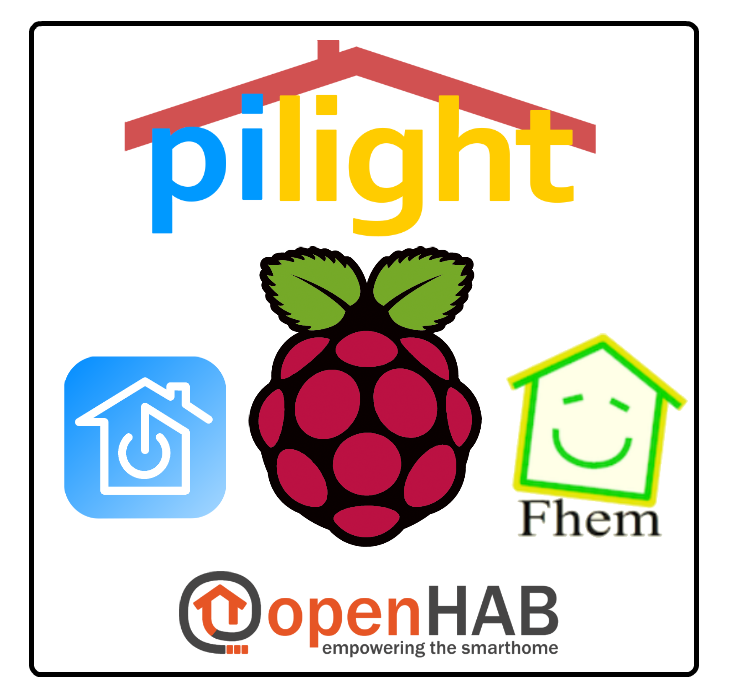
\includegraphics[width=.5\linewidth]{./include/titelbild.png}



    % examiners (Referenten)
    %\vspace*{1.5cm}
    %\Large
    \begin{center}
        \begin{tabular}[ht]{l c l}
        \iflanguage{english}{Reviewer}{Betreuer}: 
            & \hfill & \thesisreviewerone\\
        %\iflanguage{english}{Second Reviewer}{Korreferent}: 
        %    & \hfill & \thesisreviewertwo\\
        % uncomment if you want to provide info on your advisors
        %\iflanguage{english}{Advisor}{Betreuender Mitarbeiter}: 
        %    & \hfill & \thesisadvisorone\\
        %\iflanguage{english}{Second Advisor}{Zweiter betreuender Mitarbeiter}: 
        %    & \hfill & \thesisadvisortwo\\
        \end{tabular}
    \end{center}



    % working time
    \vspace{1cm}
%    \begin{center}
%        \large{{Bearbeitungszeit}: \thesistimestart \hspace*{0.25cm} -- %
%                                   \hspace*{0.25cm} \thesistimeend}
%    \end{center}



    % lowest text blocks concerning the KIT
    \begin{textblock}{10}[0,0](4,16.8)
        \tiny{KIT – Universität des Landes Baden-Württemberg und nationales Forschungszentrum in der Helmholtz-Gemeinschaft}
    \end{textblock}
    \begin{textblock}{10}[0,0](14,16.75)
        \large{\textbf{www.kit.edu}}
    \end{textblock}
\end{titlepage}

    
    \begingroup    % in order to avoid listoffigures and
    \tableofcontents                    % listoftables on new pages
    \listoffigures
    \listoftables
    \endgroup
    \cleardoublepage
    
    \MainMatter
    \chapter{Inbetriebnahme}
Im Folgenden werden die notwendigen (Installations-)Schritte zur Inbetriebnahme des Gesamtsystems auf neu installierten Betriebssystemen beschrieben.
\section{DebianVM}
Vor dem Installieren der Pakete ein Update und Upgrade durchführen:
\begin{verbatim}
$ sudo apt-get -y update 
$ sudo apt-get -y upgrade
$ sudo apt -y autoremove
\end{verbatim}

\subsection{git}
\texttt{git} wird mit \verb|$ sudo apt install git| installiert.

\subsection{Docker und Docker-Compose}
Zur Installation von Docker und Docker-Compose auf Debian zu installieren, sind folgende Schritte durchzuführen\footnote{Siehe \href{https://docs.docker.com/engine/install/debian/}{https://docs.docker.com/engine/install/debian/}}
\begin{enumerate}
	\item Pakete installieren, um das Benutzen von Repos über HTTPS zu ermöglichen: 
	\begin{verbatim}
$ sudo apt-get install \
    apt-transport-https \
    ca-certificates \
    curl \
    gnupg-agent \
    software-properties-common
\end{verbatim}
	\item GPG Schlüssel von Docker hinzufügen:
	\begin{verbatim}
	$ curl -fsSL https://download.docker.com/linux/debian/gpg \
	| sudo apt-key add 
	\end{verbatim}
	\item Mit \verb|$ sudo apt-key fingerprint 0EBFCD88| den Fingerprint des Schlüssels überprüfen. Dieser sollte \texttt{9DC8 5822 9FC7 DD38 854A E2D8 8D81 803C 0EBF CD88} entsprechen.
	\item Repository hinzufügen:
	\begin{verbatim}
	$ sudo add-apt-repository \
	"deb [arch=amd64] https://download.docker.com/linux/debian \
	$(lsb_release -cs) \
	stable"
	\end{verbatim}
	\item Docker installieren:
	\begin{verbatim}
	 $ sudo apt-get update
	 $ sudo apt-get install docker-ce docker-ce-cli containerd.io
	\end{verbatim}
	\item Docker-Compose:
	\begin{verbatim}
	sudo apt install docker-compose
	\end{verbatim}
\end{enumerate}


\subsection{MQTT/Telegraf/InfluxDB/Grafana-Container}
Das Repo mit 
\begin{verbatim}
git clone 
https://github.com/youcann/mqttTelegrafInfluxGrafana-dockerCompose.git
\end{verbatim}
herunterladen. Ins Verzeichnis wechseln und mit \verb|docker-compose up| die Container starten.

\newpage

\section{Raspberry Pi}
Vor dem Installieren der Pakete ein Update und Upgrade durchführen:
\begin{verbatim}
$ sudo apt-get -y update 
$ sudo apt-get -y upgrade
$ sudo apt -y autoremove
\end{verbatim}

\subsection{git}
\texttt{git} wird mit \verb|$ sudo apt install git| installiert.\newline
Im gewünschten Verzeichnis, z.B. im Home-Verzeichnis, das Repo mit 
\begin{verbatim}
	$ git clone https://github.com/soerman/sensordataToMQTT.git
\end{verbatim}
herunterladen. 


\subsection{Feste IP-Adresse und log2ram einstellen}
In das Repo-Verzeichnis wechseln. Im Ordner \verb|bashScripts| das Skript zum Einstellen der festen IP-Adresse (172.23.62.255) und \texttt{log2ram} mit 
\begin{verbatim}
$ bash ip_log2ram.sh
\end{verbatim}
ausführen. Anschließend den Pi neustarten.




\subsection{Docker und Docker-Compose}
Um Docker und Docker-Compose zu installieren folgende Schritte ausführen\footnote{Siehe \href{https://dev.to/rohansawant/installing-docker-and-docker-compose-on-the-raspberry-pi-in-5-simple-steps-3mgl}{https://dev.to/rohansawant/installing-docker-and-docker-compose-on-the-raspberry-pi-in-5-simple-steps-3mgl}}:
\begin{enumerate}
	\item Docker installieren:
	\begin{verbatim}
		$ curl -sSL https://get.docker.com | sh
	\end{verbatim}
	\item Berechtigung für den Nutzer \texttt{pi} erteilen, Docker-Kommandos auszuführen:
	\begin{verbatim}
		$ sudo usermod -aG docker pi
		$ newgrp docker
	\end{verbatim}
	\item Test:
	\begin{verbatim}
		$ docker run hello-world
	\end{verbatim}
	\item Abhängigkeiten installieren:
	\begin{verbatim}
		$ sudo apt-get install -y libffi-dev libssl-dev
		$ sudo apt-get install -y python3 python3-pip
		$ sudo apt-get remove python-configparser
	\end{verbatim}
	\item Docker-Compose installieren:
	\begin{verbatim}
		$ sudo pip3 -v install docker-compose
	\end{verbatim}

\end{enumerate}

\subsection{Datenlogger-Skript}
Im Verzeichnis mit den Dateien mit \verb|$ docker-compose up --build| den Docker-Container starten.

\paragraph{Anpassung}
In der \verb|docker-compose.yaml| können folgende Punkte angepasst werden:
\begin{itemize}
	\item Port an dem die Wetterstation angeschlossen ist
	\item IP-Adresse des MQTT-Servers
	\item Port des MQTT-Servers
	\item MQTT-Topic
	\item Intervall (in Sekunden) mit dem Wetterdaten abgefragt werden
	\item Pfad zum Log-File
	\item Die Log-Level, bei denen die jeweiligen Python-Logger-Handler loggen
	\item Pfad zur Datei, die zum Watchdog-Reset beschrieben werden soll
\end{itemize} 

\subsection{Watchdog}
Watchdog erst ganz zum Schluss starten, wenn das Programm ohne Probleme gestartet hat/läuft!

Im Verzeichnis \verb|bashScripts| mit 
\begin{verbatim}
$ bash watchdogStart.sh
\end{verbatim}
das Skript ausführen um den Watchdog zu starten.


\section{Webseite}
Nach erfolgreicher Inbetriebnahme ist die Webseite unter \texttt{172.23.62.107:3000} aufrufbar mit den folgenden Zugangsdaten\footnote{Lassen sich bei Erstanmeldung ändern}

\begin{verbatim}
	Benutzername: admin
	Passwort: admin
\end{verbatim}

    \chapter{Allgemeine Struktur}
Bla ganz toll die einzelnen Sachen erklären. Noch ein Blockdiagramm einfügen.
\section{Loggen der Daten}
Der Code befindet sich unter \href{https://github.com/soerman/sensordataToMQTT}{https://github.com/soerman/sensordataToMQTT} heruntergeladen werden. Im Folgenden werden kurz die einzelnen Module bzw. Klassen beschrieben.

\properparagraph{Main}
\properparagraph{dlxMetDatalogger}
\properparagraph{measurement}
\section{Webseite}    

    \Appendix
    \chapter*{\appendixname} \addcontentsline{toc}{chapter}{\appendixname}
    \section{Arbeiten mit Containern}
Um im Container Kommandos auszuführen/zu arbeiten, kann mit dem Befehl
\begin{verbatim}
docker exec -it [container-id] bash
\end{verbatim}
eine Bash-Shell im entsprechenden Container gestartet werden. Die Container-IDs der aktiven Container können mit 
\begin{verbatim}
docker ps
\end{verbatim}
aufgelistet werden.

\section{Datalogger DLx-MET}

In \autoref{tbl:anschluesse} sind die Sensoren der Wetterstation und deren jeweiliger Anschluss aufgeführt. In dieser Reihenfolge befinden sich die Daten auch im "'Array"', der geschickt wird, nachdem man einen Auslese-Befehl gesendet hat.

\begin{table}[H]
	\centering
	\caption{Anschlüsse der Sensoren an den Datenlogger}
	\label{tbl:anschluesse}
	\begin{tabularx}{0.5\textwidth}{XX}  
		\toprule
		\textbf{Sensor} & \textbf{Beschreibung} \\
		\midrule
		1 	&  Windgeschwindigkeit      	\\
		2 	&  Windrichtung 	    \\
		3   &	Temperatur 1 \\
		4   & relative Feuchtigkeit\\
		5   & Niederschlag  \\
		6   & Luftdruck \\
		7   & Einstrahlung \\
		8   & Temperatur 2\\
		\bottomrule
	\end{tabularx}
\end{table}


    %\chapter*{\appendixname} \addcontentsline{toc}{chapter}{\appendixname}
    \addcontentsline{toc}{section}{Abkürzungsverzeichnis}
    % das Abkürzungsverzeichnis entgültige Ausgeben
    \fancyhead[L]{Abkürzungsverzeichnis} %Kopfzeile links
    \newpage

    % Bibliography
    \nocite{*}
    \printbibliography[heading=bibintoc]
    %\bibliographystyle{alpha}
    %\bibliography{lit}
    % BIBTEX
    % use if you want citations to appear even if they are not referenced to: 
    % \nocite{*} or maybe \nocite{Kon64,And59} for specific entries
    %\nocite{*}

    % THEBIBLIOGRAPHY
    %\begin{thebibliography}{000}
    %    \bibitem{ident}Entry into Bibliography.
    %\end{thebibliography}
\end{document}
